% This is samplepaper.tex, a sample chapter demonstrating the
% LLNCS macro package for Springer Computer Science proceedings;
% Version 2.20 of 2017/10/04
%
\documentclass[runningheads]{llncs}
%
\usepackage{graphicx}
\usepackage{hyperref}
% Used for displaying a sample figure. If possible, figure files should
% be included in EPS format.
%
% If you use the hyperref package, please uncomment the following line
% to display URLs in blue roman font according to Springer's eBook style:
% \renewcommand\UrlFont{\color{blue}\rmfamily}

\begin{document}
\newtheorem{defi}[theorem]{Definition}
%
%\title{G2GML: Graph to Graph Mapping Language for Interoperable Use of RDF and Property Graphs}
\title{Graph to Graph Mapping Framework for Interoperable Use of RDF and Property Graphs}
%
\titlerunning{Graph to Graph Mapping Framework}
%\titlerunning{Interoperable Use of RDF and Property Graph}
% If the paper title is too long for the running head, you can set
% an abbreviated paper title here
%
\author{Hirokazu Chiba\inst{1} \and Ryota Yamanaka\inst{2} \and Shota Matsumoto\inst{3}}
%
\authorrunning{H. Chiba et al.}
% First names are abbreviated in the running head.
% If there are more than two authors, 'et al.' is used.
%
\institute{
Database Center for Life Science, Chiba 277-0871, Japan\\
\email{chiba@dbcls.rois.ac.jp}
\and
Oracle Corporation, Bangkok 10500, Thailand\\
\email{ryota.yamanaka@oracle.com}
\and
Lifematics Inc., Tokyo 101-0041, Japan\\
\email{shota.matsumoto@lifematics.co.jp}
}
%
\maketitle              % typeset the header of the contribution
%
\begin{abstract}
% The abstract should briefly summarize the contents of the paper in 15--250 words.
Increasing amounts of scientific and social data are described as graphs. As a graph data model, in addition to the standardized Resource Description Framework (RDF), the property graph model have been attracting increasing attentions.
However, interoperable management of graph data based on these data models is challenging due to the differences in data models and formats depending on verious implementations.
Here, we redefine the property graph model incorporating the differences in the existing models and propose interoperable serialization formats for property graphs. These formats can be converted into specific formats for each of the databases mentioned above. We also developed a general framework for mapping RDF graphs to property graphs on the basis of the Graph to Graph Mapping Language (G2GML).
Using this framework, graph data described in the RDF model can be converted to the property graph model and can be loaded to several graph database engines for further analysis. 
%This work provides interoperability not only between property graph formats but also between RDF and proper graphs.
%Future works include implementing and utilizing graph algorithms to make the most of the accumulated data in various analytical engines.

\keywords{RDF \and Property Graph \and Graph Database}
\end{abstract}

\section{Introduction}
% Please note that the first paragraph of a section or subsection is not indented. The first paragraph that follows a table, figure, equation etc. does not need an indent, either.

Increasing amounts of scientific and social data are described as graphs. As a format of graph data, the Resource Description Framework (RDF)~\cite{rdf} is widely used. 
% Although RDF data can be queried using the SPARQL language~\cite{sparql} in a flexible way, SPARQL is not dedicated to traversal of graphs and has a limitation in implementing graph analysis algorithms.
In the context of graph analysis, the property graph model~\cite{angles1,angles} have been attracting increasing attentions. Various graph database engines, including Neo4j~\cite{neo4j}, Oracle Labs PGX~\cite{pgx}, and Amazon Neptune~\cite{neptune}, adopt this model. These graph database engines support algorithms for traversal or analyzing graphs. However, currently not many datasets are consistently described in the property graph model, so the application of these powerful engines are limited.

Considering this situation, it is valuable to develop a method to transform RDF data into property graphs. However, the transformation is not straightforward due to the differences in the data model. 
In RDF graphs, all information is expressed as the triple (node-edge-node), whereas in property graphs, arbitrary information can be contained in each of the nodes and edges as key-value form. 
Although previous works addressed this issue by formalizing transformations~\cite{hartig},
users cannot define their specific mappings intended for each use case.

Here, we define the property graph model independent of specific graph database implementations and also developed a framework based on the Graph to Graph Mapping Language (G2GML) for mapping RDF graphs to property graphs. Using this framework, accumulated graph data described in the RDF model can be converted to the property graph model and can be loaded to several graph database engines. 


\section{The Property Graph Model}
Here, we define the property graph model independent of specific graph database implementations. For the purpose of interoperability, we incorporate differences in property graph models, taking into consideration multiple labels or property values for nodes and edges, as well as mixed graphs with both of directed and undirected edges. The property graph model we redefine here requires the following characteristics:

\begin{itemize}
    \item A property graph contains nodes and edges.
    \item Each of the nodes and edges can have zero or more labels.
    \item Each of the nodes and edges can have properties (key-value pairs).
    \item Each property can have multiple values.
    \item Each edge can be directed or undirected.
\end{itemize}
More formally, we define the property graph model as follows.

\begin{defi}[Property Graph Model]
\leavevmode \vspace{1mm} \\
A \emph{Property Graph} is a tuple
$PG = \langle N, E_d, E_u, S, V, P, e, l_n, l_e, p_n, p_e\rangle$, where:
\begin{enumerate}
    \item $N$ is a set of nodes.
    \item $E_d$ is a set of directed edges.
    \item $E_u$ is a set of undirected edges.
    \item $E$ is a set of edges where $E = E_d \cup E_u$.
    \item $S$ is a set of strings.
    \item $V$ is a set of values of arbitrary data types.
    \item $P$ is a set of properties. Each property has the form $p = \langle k,v \rangle$, where $k \in S$ and $v \in 2^V$.
    \item $e: E \to \langle N \times N \rangle$ is a function which yields the endpoints of each directed or undirected edge (if the edge is directed, the first node is the source and the second node is the destination).
    \item $l_n : N \to 2^S$ is a function mapping each node to its multiple labels.
    \item $l_e : E \to 2^S$ is a function mapping each edge to its multiple labels.
    \item $p_n : N \to 2^P$ is a function used to assign nodes to their multiple properties.
    \item $p_e : E \to 2^P$ is a function used to assign edges to their multiple properties.
\end{enumerate}
\end{defi}


\section{Serializing Property Graphs}
According to our definition of the property graph model, we propose serialization in flat text and JSON. The flat text format (PG) is better for human readability and line-oriented processing, while the JSON format (JSON-PG) is best used for server-client communication.

The flat text PG format has the following characteristics, and an example is given in Figure~\ref{fig:example-pg}.

\begin{itemize}
    \item Each line describes a node or an edge.
    \item All elements in each line are separated by space or tab.
    \item In each of the node lines, the first column contains the node ID.
    \item In each of the edge lines, the first three columns contain the source node ID, the direction, and the destination node ID.
    \item Each line can contain an arbitrary number of labels.
    \item Each line can contain an arbitrary number of properties (key-value pairs).
\end{itemize}

More formally, we describe the PG format in the EBNF notation as follows.

\begin{defi}[PG Format]
\leavevmode \vspace{1mm} \\
\emph{EBNF notation of the PG format.}
\begin{scriptsize}
\begin{verbatim}
    PG         ::= (Node | Edge)+
    Node       ::= NODE_ID Labels Properties NEWLINE
    Edge       ::= NODE_ID Direction NODE_ID Labels Properties NEWLINE
    Labels     ::= Label*
    Properties ::= Property*
    Label      ::= ':' STRING
    Property   ::= STRING ':' Value
    Value      ::= STRING | NUMBER
    Direction  ::= '--' | '->'
\end{verbatim}
\end{scriptsize}
\end{defi}

Next, we describe the JSON-PG format which follows the JSON syntax in addition to the above definition of the property graph model. The JSON-PG format has the following characteristics, and an example of the format is shown in Figure~\ref{fig:example-json}. It is to be noted that, whereas the set of labels or property values are represented as arrays in JSON, those elements are supposed to have no specific order according to the the property graph model.

\begin{itemize}
    \item Nodes and edges are listed under \texttt{nodes} and \texttt{edges} elements, respectively.
    \item Edge direction is defined with the boolean element \texttt{undirected}. By default it is false (directed).
    \item Labels are listed under the \texttt{labels} element.
    \item Properties (key-value pairs) are listed under the \texttt{properties} element.
\end{itemize}

Furthermore, we have implemented command-line tools to convert between PG and JSON-PG, as well as to transform them into formats for well-known graph databases such as Neo4j, Oracle Labs PGX, and Amazon Neptune. The practical use cases of our tools demonstrate that the proposed data model and formats have the capability to describe property graph data begin used in existing graph databases (see \url{https://github.com/g2glab/pg}).

\begin{figure}[!t]
\begin{scriptsize}
\begin{verbatim}
# NODES
101  :Person  name:Alice  age:15  country:"United States"
102  :Person  :Student  name:Bob  country:Japan  country:Germany

# EDGES
101 -- 102  :sameSchool  :sameClass  since:2012
102 -> 101  :likes  since:2015
\end{verbatim}
\end{scriptsize}
\caption{Example of PG}
\label{fig:example-pg}
\end{figure}

\begin{figure}[!t]
\begin{scriptsize}
\begin{verbatim}
{
  "nodes":[
    {
     "id":101,
     "labels":["Person"],
     "properties":{"name":["Alice"], "age":[15], "country":["United States"]}
    },
    {
     "id":102,
     "labels":["Person", "Student"],
     "properties":{"name":["Bob"], "country":["Japan", "Germany"]}
    }
  ],https://ja.overleaf.com/project/5d6e87b11a254100014e487d
  "edges":[
    {
     "from":101,
     "to":102,
     "undirected":true,
     "labels":["sameSchool", "sameClass"],
     "properties":{"since":[2012]}
    },
    {
     "from":102,
     "to":101,
     "labels":["likes"],
     "properties":{"since":[2015]}
    }
  ]
}
\end{verbatim}
\end{scriptsize}
\caption{Example of JSON-PG}
\label{fig:example-json}
\end{figure}


\section{Mapping RDF graphs to Property Graphs}

Here, we developed a framework for mapping RDF to property graphs.
Figure~\ref{fig:dataflow} shows the overview of proposed framework.
In the proposed framework, users write mappings from RDF graphs to property graphs in G2GML.
This mapping can be processed by an implementation called \textit{G2G Mapper}, which is implemented by authors (available on \url{https://github.com/g2gml}). This tool retrieves RDF data from SPARQL endpoints and converts them to property graph data in several different formats specified by popular graph databases.

G2GML is a declarative language which consists of pairs of RDF graph patterns and property graph patterns. 
An intuitive meaning of a G2GML is a mapping between RDF subgraphs that matches the described patterns and described components of the property graph. In the next section, we briefly explain the syntax of G2GML with a concrete example usage.

\begin{figure}
\center
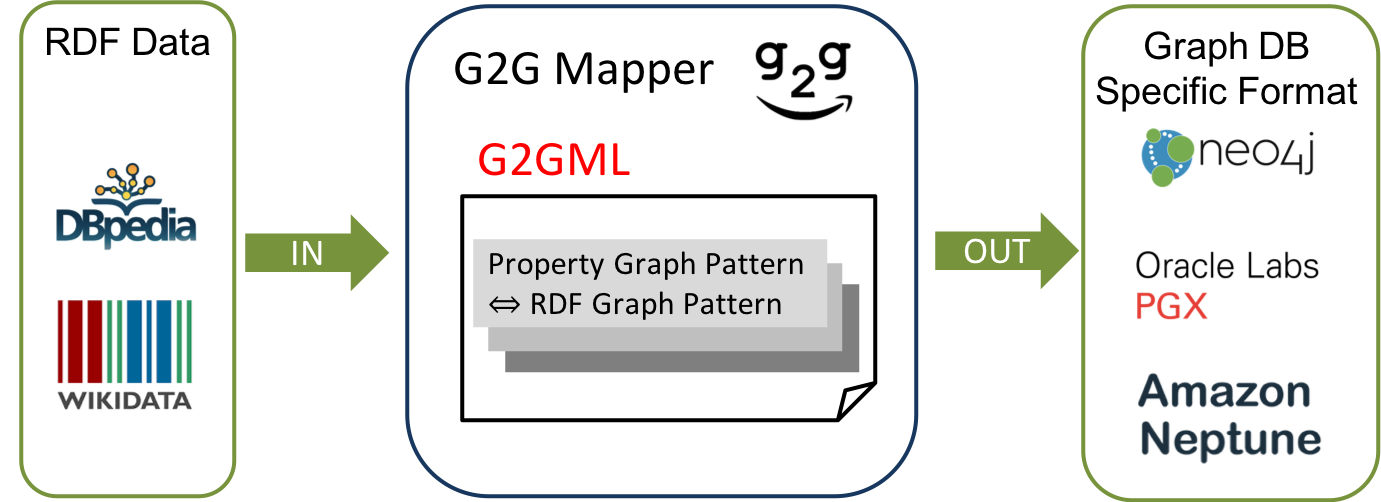
\includegraphics[width=1.0\textwidth]{dataflow.png}
\caption{Overview of the graph to graph mapping}
\label{fig:dataflow}
\end{figure}

%\subsection{Usecase}

Figure~\ref{fig:conversion} shows an example of G2GML mapping, which converts RDF data retrieved from DBpedia into property graph data. When we focus on relationships that one musician and another are in the same group, the information can be summarized into the property graph data as shown in this figure.

\begin{figure}
\center
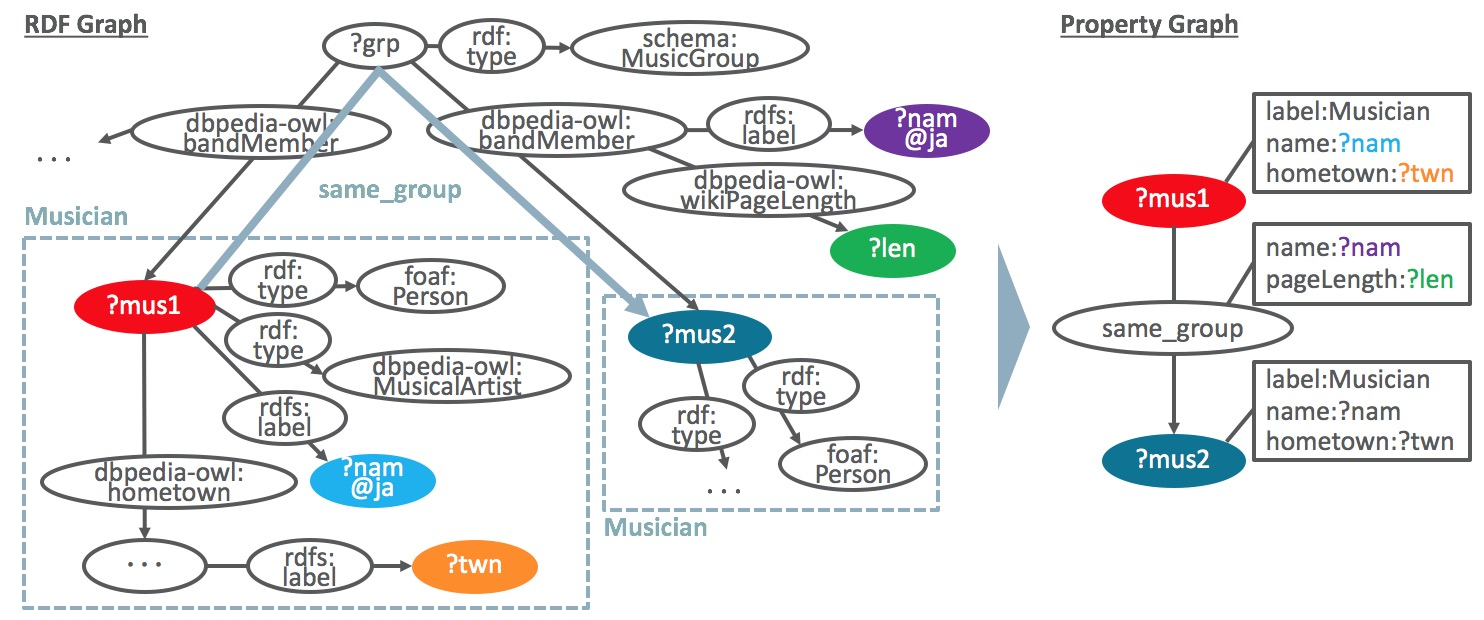
\includegraphics[width=1.0\textwidth]{example.jpg}
\caption{Schematic example of graph to graph mapping}
\label{fig:conversion}
\end{figure}

For this conversion, the actual G2GML is described as in Figure~\ref{fig:g2gml}. It starts with URI prefixes used to write mappings, and then, each mapping consists of one unindented line of a property graph pattern and indented lines of an RDF graph pattern. A property graph pattern is written in a syntax like Cypher (the query language of Neo4j), whereas an RDF graph pattern is written as a pattern in SPARQL. Variables in each pattern are mapped by those names. This example contains one node mapping for \texttt{Musician} entity and one edge mapping for \texttt{same\_group} relationship only. In G2GML, edge mappings are defined based on the conditions of node mappings, which means that edges are generated in property graph iff both nodes' patterns and edges' patterns are matched in RDF graph. Also, \texttt{mus, nam, dat, twn} and \texttt{len} are used as variables to extract resources and literals from RDF graph. In the resulting property graph, resources can be mapped to nodes, while literals can be mapped to values of properties.

\begin{figure}[!t]
\vspace{2mm}
\begin{scriptsize}
\begin{verbatim}
# Prefixes
PREFIX rdf: <http://www.w3.org/1999/02/22-rdf-syntax-ns#>
PREFIX rdfs: <http://www.w3.org/2000/01/rdf-schema#>
PREFIX prop: <http://dbpedia.org/property/>
PREFIX schema: <http://schema.org/>
PREFIX dbpedia-owl: <http://dbpedia.org/ontology/>
PREFIX foaf: <http://xmlns.com/foaf/0.1/>

# Node mapping
(mus:Musician {vis_label:nam, born:dat, hometown:twn})                    # PG Pattern
    ?mus rdf:type foaf:Person, dbpedia-owl:MusicalArtist .                # RDF Pattern
    ?mus rdfs:label ?nam .
    OPTIONAL { ?mus prop:born ?dat }
    OPTIONAL { ?mus dbpedia-owl:hometown / rdfs:label ?twn }

# Edge mapping
(mus1:Musician)-[:same_group {label:nam, length:len}]->(mus2:Musician)    # PG Pattern
    ?grp a schema:MusicGroup ;                                            # RDF Pattern
         dbpedia-owl:bandMember ?mus1 , ?mus2 .
    FILTER(?mus1 != ?mus2)
    OPTIONAL { ?grp rdfs:label ?nam. FILTER(lang(?nam) = "ja")}
    OPTIONAL { ?grp dbpedia-owl:wikiPageLength ?len }
\end{verbatim}
\end{scriptsize}
\caption{Example of G2GML}
\label{fig:g2gml}
\end{figure}

Finally, Figure~\ref{fig:sparql} shows the SPARQL query to retrieve the pairs of musicians who are in the same group. After G2GML mapping above, we can load the generated property graph data into graph databases, such as Oracle Labs PGX, and the query can be written in PGQL~\cite{pgql} (the query language of PGX).

\begin{figure}[!t]
\vspace{2mm}
\begin{scriptsize}
\begin{verbatim}
# SPARQL
PREFIX rdf: <http://www.w3.org/1999/02/22-rdf-syntax-ns#>
PREFIX rdfs: <http://www.w3.org/2000/01/rdf-schema#>
PREFIX schema: <http://schema.org/>
PREFIX dbpedia-owl: <http://dbpedia.org/ontology/>
SELECT DISTINCT
    ?nam1 ?nam2
WHERE {
    ?mus1 rdf:type foaf:Person , dbpedia-owl:MusicalArtist .
    ?mus2 rdf:type foaf:Person , dbpedia-owl:MusicalArtist .
    ?mus1 rdfs:label ?nam1 . FILTER(lang(?nam1) = "ja") .
    ?mus1 rdfs:label ?nam2 . FILTER(lang(?nam2) = "ja") .
    ?grp a schema:MusicGroup ;
         dbpedia-owl:bandMember ?mus1 , ?mus2 .
    FILTER(?mus1 != ?mus2)
}

# PGQL
SELECT DISTINCT m1.name, m2.name WHERE (m1)-[same_group]-(m2)
\end{verbatim}
\end{scriptsize}
\caption{Example of SPARQL and PGQL queries}
\label{fig:sparql}
\end{figure}

\section{Discussion}
The graph data have been attracting increasing attentions recently. 
So far, there have been implementations of graph databases on the basis of various data models and query languages. 
There are community-based activities for standardizing graph query language for interoperable use of property graph databases~\cite{angles3}. Similarly, standardization of the property graph model with support for various database implementations will enhance the interoperable use of graph data. In fact, there is a need for graph standardization in the community and graph data standardization was recently discussed in a workshop~\cite{w3c}. There is a similar proposals for property graph model and serialization~\cite{tomaszuk} and it is noteworthy that two independent approach converges to the similar solution. Our serialization already has an implementation for some of the major database engines and has a potential to cover further various implementations. %However, it requires developing a converter for each format. 
This work provides a basis of an interoperable platform for creating, exchanging, and utilizing property graph data.

As related works, there were efforts to develop a method to convert relational to graph database~\cite{virgilio1}. Given that now RDF has prevailed as a standardized data model in scientific communities, considering the mapping on the basis of the standardized RDF is crucial. There were discussions about the interoperability on RDF and property graph model~\cite{hartig,das,thakkar}. There were efforts to develop a method to convert RDF into property graphs~\cite{tomaszuk1,virgilio}. However, due to the flexibility in terms of what kind of information can be expressed by each edge in property graphs, there was a need for controllability for the mapping. But there was not a method for controlled mapping from RDF to property graphs.
To the best of our knowledge, this is a first attempt to develop a general framework for mapping between RDF and property graphs. The G2GML we have designed is a declarative mapping language. As a merit of declarative description, we can concentrate on the logic of the mapping. In the sense that the mapping crerates graph patterns on the basis of matches to exsisting graph patterns, it has relation to semantic inference. Similar concept can be found in SPARQL construct query. While the SPARQL construct is mapping on the same data model, G2GML defines mapping between different data modesl. Currently, it is limited to the mapping from RDF to property graphs, it can be extended to the mapping from property graph to RDF. However, if mapping includes the SPARQL pattern that are not declarative, it is not applicable for generating RDF triples.

%Future works include further analysis of the converted graph data on the database engines adopting the property graph model.

\section{Conclusion}
We propose the property graph model independent of specific graph database implementations and working prototype for serialization formats based on the data model.
We defined G2GML for mapping RDF graphs to property graphs and implemented a converter based on the G2GML.
Our data model and mapping framework will increase the interoperability of existing graph databases and make it easier for users to create, exchange, and utilize property graph data.

\section*{Acknowledgements}
Part of the work was conducted through the BioHackathon meetings (\url{http://www.biohackathon.org}). We thank Yuka Tsujii for helping creating figures. We thank Ramona Roess for careful review of the manuscript and useful comments.

%
% ---- Bibliography ----
%
% BibTeX users should specify bibliography style 'splncs04'.
% References will then be sorted and formatted in the correct style.
%
% \bibliographystyle{splncs04}
% \bibliography{mybibliography}
%
\begin{thebibliography}{8}

\bibitem{rdf}
RDF 1.1 Concepts and Abstract Syntax, W3C Recommendation 25 February 2014, \url{http://www.w3.org/TR/rdf11-concepts/}.

\bibitem{sparql}
SPARQL 1.1 Query Language, W3C Recommendation 21 March 2013, \url{http://www.w3.org/TR/sparql11-query/}.

\bibitem{angles1}
Angles, R., Gutierrez, C.: An introduction to Graph Data Management. arXiv preprint arXiv:1801.00036 (2017)

\bibitem{angles}
Angles, R., Arenas, M., Barceló, P., Hogan, A., Reutter, J., Vrgoc, D.: Foundations of Modern Query Languages for Graph Databases. ACM Computing Surveys (CSUR), 50(5), 68 (2017)

\bibitem{neo4j}
The Neo4j Graph Platform, \url{https://neo4j.com/}.

\bibitem{pgx}
Oracle Labs Parallel Graph AnalytiX (PGX), \url{https://www.oracle.com/technetwork/oracle-labs/parallel-graph-analytix/overview/index.html}.

\bibitem{neptune}
Amazon Neptune, \url{https://aws.amazon.com/neptune/}.

\bibitem{pgql}
van Rest, O., Hong, S., Kim, J., Meng, X., Chafi, H.: PGQL: a property graph query language. In Proceedings of the Fourth International Workshop on Graph Data Management Experiences and Systems (p. 7). ACM. (2016)

\bibitem{w3c}
W3C Workshop on Web Standardization for Graph Data, \url{https://www.w3.org/Data/events/data-ws-2019/}

\bibitem{tomaszuk}
Tomaszuk D., Angles R., Szeremeta Ł., Litman K., Cisterna D.:
Serialization for property graphs. International Conference: Beyond Databases, Architectures and Structures, 57-69 (2019)

\bibitem{angles3}
Angles, R., Arenas, M., Fletcher, G. H., Gutierrez, C., Lindaaker, T., Paradies, M., ... , Voigt, H.: G-CORE: A Core for Future Graph Query Languages. arXiv preprint arXiv:1712.01550 (2017)

\bibitem{hartig}
Hartig, O.: Reconciliation of RDF* and property graphs. arXiv preprint arXiv:1409.3288 (2014)

\bibitem{das}
Das, S., Srinivasan, J., Perry, M., Chong, E. I., Banerjee, J.: A Tale of Two Graphs: Property Graphs as RDF in Oracle. In EDBT (pp. 762-773) (2014)

\bibitem{thakkar}
Thakkar, H., Punjani, D., Keswani, Y., Lehmann, J., Auer, S.: A Stitch in Time Saves Nine--SPARQL querying of Property Graphs using Gremlin Traversals. arXiv preprint arXiv:1801.02911 (2018)

\bibitem{virgilio1}
De Virgilio, R., Maccioni, A., Torlone, R.: Converting relational to graph databases. In First International Workshop on Graph Data Management Experiences and Systems (p. 1). ACM. (2013)

\bibitem{tomaszuk1}
Tomaszuk, D.: RDF Data in Property Graph Model. In Metadata and Semantics Research: 10th International Conference, MTSR 2016, Göttingen, Germany, November 22-25, 2016, Proceedings (pp. 104-115). Springer International Publishing (2016)

\bibitem{virgilio}
De Virgilio, R.: Smart rdf data storage in graph databases. In Proceedings of the 17th IEEE/ACM International Symposium on Cluster, Cloud and Grid Computing (pp. 872-881). IEEE Press. (2017)

% \bibitem{ref_article1}
% Author, F.: Article title. Journal \textbf{2}(5), 99--110 (2016)

% \bibitem{ref_lncs1}
% Author, F., Author, S.: Title of a proceedings paper. In: Editor,
% F., Editor, S. (eds.) CONFERENCE 2016, LNCS, vol. 9999, pp. 1--13.
% Springer, Heidelberg (2016). \doi{10.10007/1234567890}

% \bibitem{ref_book1}
% Author, F., Author, S., Author, T.: Book title. 2nd edn. Publisher,
% Location (1999)

% \bibitem{ref_proc1}
% Author, A.-B.: Contribution title. In: 9th International Proceedings
% on Proceedings, pp. 1--2. Publisher, Location (2010)

% \bibitem{ref_url1}
% LNCS Homepage, \url{http://www.springer.com/lncs}. Last accessed 4
% Oct 2017
\end{thebibliography}
\end{document}
